\section{Theorie}
\label{sec:Theorie}
\subsection{Beugung allgemein}
Klassisch kann man die Entstehung von Beugungsmustern an einem Spalt durch das Huygenssche Prizip erklären.
Dieses besagt, dass ein an jeder Position einer Wellenfront eine neue Kugelwelle entsteht.
Aus der Intensitätsverteilung kann man auf die Gestalt des Objektes, an dem das Licht gebeugt wird, auch Aperturfunktion genannt, schließen.
Die Funktion der Intensitätsverteilung kann, unter bestimmten Voraussetzungen, in die Aperturfunktion überführt werden und umgekehrt.

\subsection{Fresnelsche und Frauenhofer Beugung}
Wenn Beugung beobachtet wird, wird zwischen der Fresnelnelschen Beugung und der Frauenhofer Beugung unterschieden.
Bei der Fresnelnelschen Beugung liegt die Lichtquelle im Endlichen, wie in \ref{fig:Fresnel} dargestellt.
Hier sind die Winkel, mit denen die Lichtstrahlen eintreffen, unterschiedlich. 
Das hat zur Folge, dass die Strahlen, die im Aufpunkt P auftreffen, auch verschiedene Beugungswinkel $\varphi$ aufweisen.

\begin{figure}[H]
    \centering
    \caption{Abgebildet ist die grafische Darstellung der Fresnel-Beugung am Einzelspalt.}
    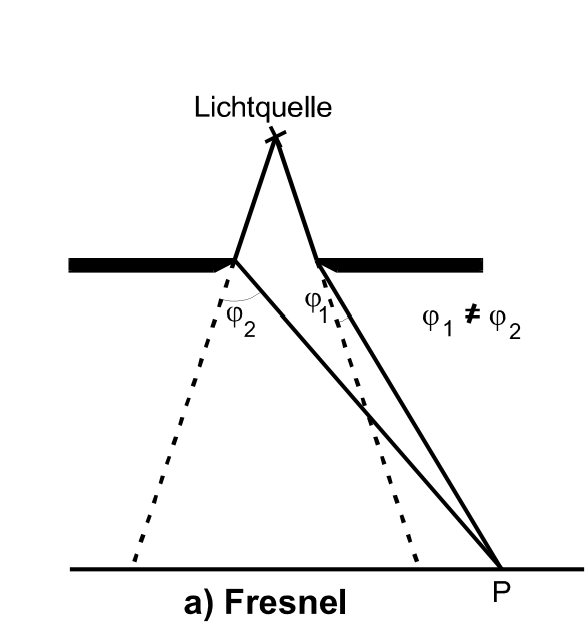
\includegraphics{Bilder/Fresnel.png}
    \label{fig:Fresnel}
\end{figure}

Bei der Frauenhofer Beugung liegt die Lichtquelle im Unendlichen, was zur Auswirkung hat, dass die auf den Spalt treffenden Strahlen parallel sind.
Somit ist auch der Beugungswinkel von Strahlen, welche durch eine Sammellinse, wie in \ref{fig:Frauenhofer} abgebildet, auf einen Aufpunkt P fokussiert werden und dort interferieren, identisch.
Im folgenden Versuch wird die Frauenhofer Beugung behandelt, da diese mathematisch einfacher ist.

\begin{figure}[H]
    \centering
    \caption{Hier wird ein Schema der Fresnel-Beugung am Einzelspalt gezeigt.}
    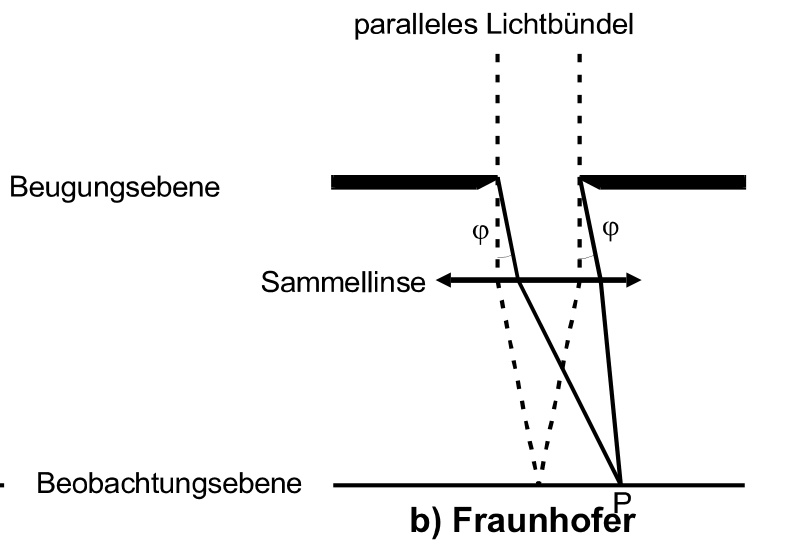
\includegraphics{Bilder/Frauenhofer.png}
    \label{fig:Frauenhofer}
\end{figure}

\subsection{Intensitätsverteilung}
Wenn eine Ebene Welle mit der Feldstärke
\begin{equation}
    A(z,t)=A_0 e^{i(\omega t - \frac{2 \pi z}{\lambda} )}
    \label{eqn:Feldstärke}
\end{equation}
pro Längeneinheit auf einen Einzelspalt trifft, welcher deutlich höher ist als breit, ergibt sich durch Kombination vom Huygensschen Prinzip und der Frauenhofer Beugung eine Amplitudenverteilung.
Diese hat die Form 
\begin{equation}
    B(\varphi)=A_0 b \frac{\sin \eta}{\eta}
    \label{eqn:Amplitude}
\end{equation}
 .
 Dabei ist 
 \begin{equation}
    \eta = \frac{\pi b \sin{\varphi}}{\lambda}
 \end{equation}
Wenn die Amplitude in Abhängigkeit zum Beugungswinkel aufgetragen wird, ergibt sich eine Verteilung wie in \ref{fig:Amplitude} gezeigt.


 \begin{figure}[H]
    \centering
    \caption{Abgebildet ist die Amplitudenverteilung einer ebenen Welle, die an einem Parallelspalt gebeugt wird.}
    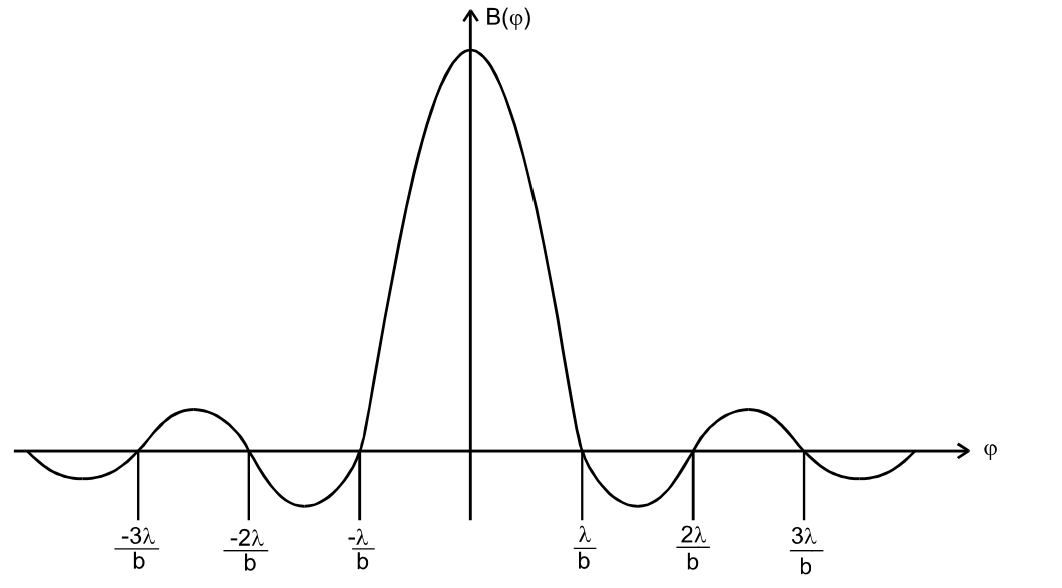
\includegraphics{Bilder/Amplitude.png}
    \label{fig:Amplitude}
\end{figure}

Die Intensität von Photonen ist proportional zum Quadrat der Amplitude und lässt sich hier über 
\begin{equation}
    I(\varphi)=A_0^2 b^2 \biggl( \frac{\lambda}{\pi b \sin{varphi}}\biggr)^2 \cdot \sin^2 \biggl( \frac{\pi b \sin(\varphi)}{\lambda}\biggr)
    \label{fig:Intensität}
\end{equation}
berechnen.

Bei einem Doppelspalt gitl für die Intensität
\begin{equation}
    I(\varphi)=4 \cos^2(\frac{\pi s \sin}) b^2 \biggl( \frac{\lambda}{\pi b \sin \varphi}\biggr)^2 \cdot \sin^2 \biggl( \frac{\pi b \sin \varphi}{\lambda}\biggr)
    \label{fig:Intensität2}
\end{equation}